\documentclass{standalone}

\usepackage{graphics}
\usepackage[dvipsnames,svgnames]{xcolor}

\usepackage{tikz,pgf,pgfplots,circuitikz}
\pgfplotsset{compat=1.15}
\usetikzlibrary{intersections,arrows.meta,angles,calc,3d,decorations.pathmorphing}

\usepackage{amssymb,amsfonts,amsthm,mathtools}
\usepackage{physics,braket,bm}

\begin{document}  
  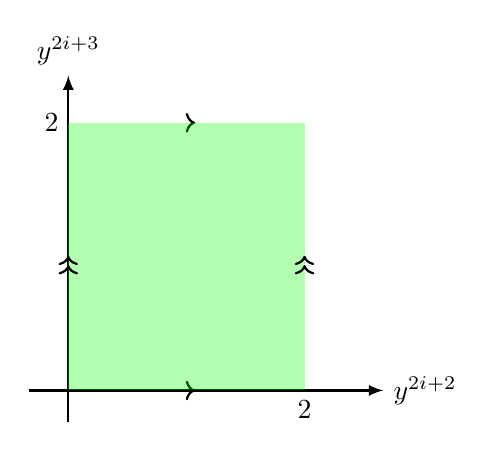
\begin{tikzpicture}[scale=1]
    \draw[->,thick](1.6,0)--(1.61,0);
    \draw[->,thick](1.6,3.4)--(1.61,3.4);

    \draw[-latex,thick](-0.5,0)--(4,0) node[right]{$y^{2i+2}$};
    \draw[-latex,thick](0,-0.4)--(0,4) node[above]{$y^{2i+3}$};

    \fill [green,opacity=0.3] (0,0)--(3.0,0)--(3.0,3.4)--(0.0,3.4);

    \draw[->>,thick](0,1.7)--(0,1.71);
    \draw[->>,thick](3,1.7)--(3,1.71);

    \draw (3,0)node [below]{$2$};
    \draw (0,3.4)node [left]{$2$};
  \end{tikzpicture}
\end{document}
